\documentclass{report}
\usepackage[utf8]{inputenc}
\usepackage[francais]{babel}
\usepackage[T1]{fontenc}
\usepackage{listings}
\usepackage{graphicx}
\usepackage{hyperref}
\usepackage{titlesec}
\usepackage{amsmath}
\usepackage{color}
\setcounter{tocdepth}{5}
\setcounter{secnumdepth}{4}
\definecolor{dkgreen}{rgb}{0,0.6,0}
\definecolor{gray}{rgb}{0.5,0.5,0.5}
\definecolor{mauve}{rgb}{0.58,0,0.82}
\definecolor{gray}{rgb}{0.4,0.4,0.4}
\definecolor{darkblue}{rgb}{0.0,0.0,0.6}
\titleformat{\paragraph}
{\normalfont\normalsize\bfseries}{\theparagraph}{1em}{}
\titlespacing*{\paragraph}
{0pt}{3.25ex plus 1ex minus .2ex}{1.5ex plus .2ex}
\renewcommand{\thesection}{\Roman{section}}
\hypersetup{
    colorlinks=true,
    linkcolor=black,
    filecolor=magenta,
    urlcolor=cyan,
}
\lstnewenvironment{cc}
{
\lstset{frame=tblr,
  language=C,
  aboveskip=3mm,
  belowskip=3mm,
  showstringspaces=false,
  columns=flexible,
  basicstyle={\small\ttfamily},
  numbers=none,
  numberstyle=\tiny\color{gray},
  keywordstyle=\color{blue},
  commentstyle=\color{dkgreen},
  stringstyle=\color{mauve},
  breaklines=true,
  breakatwhitespace=true,
  tabsize=3
}}
{}

\begin{document}
\title{
  \begin{minipage}\linewidth
      \centering
      Projet AOA sujet 10
      \vskip 5pt
      \author{
        ALEXANDRE Julien \\
        \texttt{julien.alexandre@isty.uvsq.fr}
      \and
        VIRLOGEUX Marin \\
        \texttt{marin.virlogeux@isty.uvsq.fr}
      \and
        LEDOYEN Paul \\
        \texttt{paul.ledoyen@isty.uvsq.fr}
      \and
        DRISSI Mohamed Reda \\
        \texttt{reda-mohamed@isty.uvsq.fr}
      }
    \end{minipage}
}
\maketitle
\newpage
\tableofcontents
\newpage
\section{Introduction}
  \subsection{Specs de la machine utilisée}
    \begin{itemize}
      \item CPU : \href{https://ark.intel.com/products/88195/Intel-Core-i7-6700K-Processor-8M-Cache-up-to-4_20-GHz}
        {intel core i7 6700K 4.0GHZ 4 physical cores, 8 logical(HyperThreading©) turbo boost off}
      \item RAM : Corsair CMK16GX4M2B3000C15 Vengeance LPX 16GB DDR4 3000MHz C15 XMP 2.0
      \item Stockage : \href{http://downloadcenter.samsung.com/content/UM/201711/20171115103115156/Samsung_SSD_850_PRO_Data_Sheet_Rev_3.pdf}
          {Samsung 850 PRO SSD 512GB}
    \end{itemize}
    \subsection{Système}
      \begin{itemize}
      \item OS : Debian 9.4 Stretch (stable) x86\_64
      \item Kernel :  4.9.0-6-amd64
      \item gcc : 6.3.0 20170516 (Debian 6.3.0-18+deb9u1)
      \item icc : 18.0.1 20171018
    \end{itemize}
  \subsection{Topologie du système}
    \begin{figure}[ht!]
      \centering
      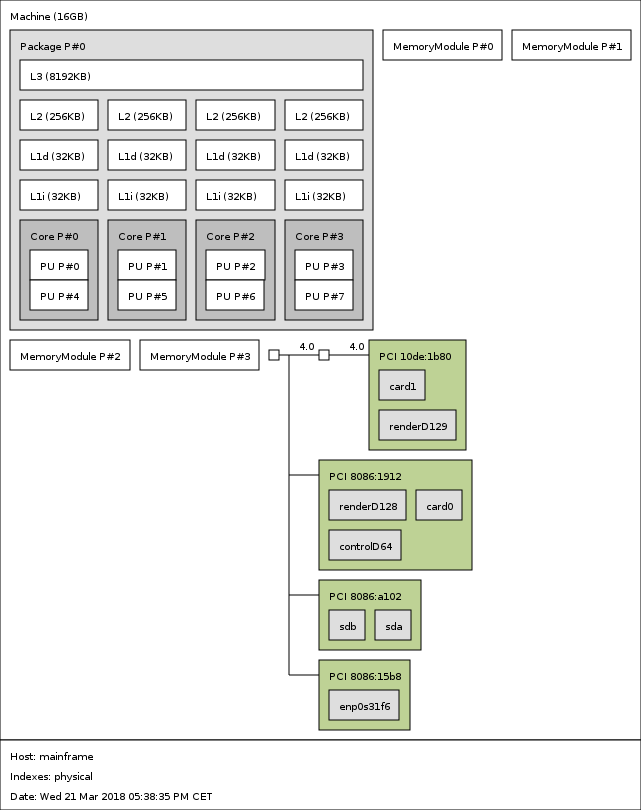
\includegraphics[scale=0.35]{resources/lstopo.png}
      \caption{Topologie générée par \href{https://manpages.debian.org/jessie/hwloc/lstopo.1.en.html}{lstopo}}
    \end{figure}
  \newpage
  \subsection{Code de la boucle}
    \lstinputlisting[language=c]{../subject10.c}
\section{Determination des paramètres}
  \subsection{Taille des données}
    Notre boucle utilise un tableau de \texttt{double} de taille $n\times n$
    chaque case prend 8 octets. \\
    Donc le coût total (en mémoire) de notre boucle sera de $4n^2$ . \\

    Si nous voulons utiliser L1, L2, L3 ou la ram il faut trouver l'intervalle de chacun
    Soit T la taille maximale (qui serait en puissance de 2 alors $T=2^t$) :
    \begin{align}
      4n^2 \leq 2^t \\
      n \leq 2^{\frac{t-2}{2}}
    \end{align}
    Les données des différents caches et ram sont
    \begin{itemize}
      \item L1 : 32Ko   = $2^{15}$ octets
      \item L2 : 256Ko  = $2^{18}$ octets
      \item L3 : 8192Ko = $2^{23}$ octets
      \item RAM: 16Gb   = $2^{34}$ octets
    \end{itemize}
    \vspace{5mm}
    \begin{tabular}{|l| c | c | c|}
      \hline
      Mémoire & $2^t$ & Taille & coût \\\hline
      \hline
      L1 & 15 & 90 & 31.64Ko \\\hline
      L2 & 18 & 256 & 256Ko \\\hline
      L3 & 23 & 1448 & 8190Ko \\\hline
      RAM & 34 & 65536 & 16Gb \\\hline
    \end{tabular}
    \subsection{Déterminer le warmup}
    \subsubsection{L1 : taille 90}
    \subsubsection{L2 : taille 256}
    \subsubsection{L3 : taille 1448}
    \subsubsection{RAM : taille 65536}
\end{document}
